\subsection{Person 6 – SUS 85}  
\textbf{Zur Person:}\\
Logistikmitarbeiterin, 65 Jahre alt  

\textbf{Beobachtung:}  
\begin{enumerate}
    \item Zeichnen Sie frei für etwa 2 Minuten.
    \begin{itemize}
        \item Kein Problem.
    \end{itemize}

    \item Löschen Sie Ihre Zeichnung vollständig.
    \begin{itemize}
        \item Rotieren als Undo verwechselt.  
        \item Trash-Icon nicht gesehen.
    \end{itemize}

    \item Laden Sie die PDF-Datei mit dem Grundriss hoch.
    \begin{itemize}
        \item Zuerst in Windows-Taskleiste geschaut.  
        \item Danach klar und kein Problem.
    \end{itemize}

    \item Ändern Sie die Stiftfarbe auf Rot.
    \begin{itemize}
        \item Hat Radiergummi ausgewählt, da gedacht, Stift würde Schrift öffnen.
    \end{itemize}

    \item Suchen Sie \texttt{BEDROOM3} und zeichnen Sie einen Tisch links vom Bett.
    \begin{itemize}
        \item Sucht nach einem Symbol, um Tisch einzufügen.  
        \item Nach kleiner Anweisung kein Problem.
    \end{itemize}

    \item Radieren Sie den Tisch und zeichnen Sie ihn rechts vom Bett.
    \begin{itemize}
        \item Findet es nicht schön, dass Hintergrund „mitgegümmelt“ wird.  
        \item Sehr kleiner Tisch gezeichnet, Problem beim genauen Beschriften.  
    \end{itemize}

    \item Zeichnen Sie die Abmessungen 1\,m $\times$ 1\,m und schreiben Sie «table» hinein.
    \begin{itemize}
        \item Schreiben bei Aufgabe 1 ging bereits gut.
        \item Kein Problem.
    \end{itemize}

    \item Speichern Sie den Plan auf Ihrem Laptop.
    \begin{itemize}
        \item Kein Problem.
    \end{itemize}
\end{enumerate}

\clearpage

\textbf{SUS-Antworten (Bild):}
\begin{center}
    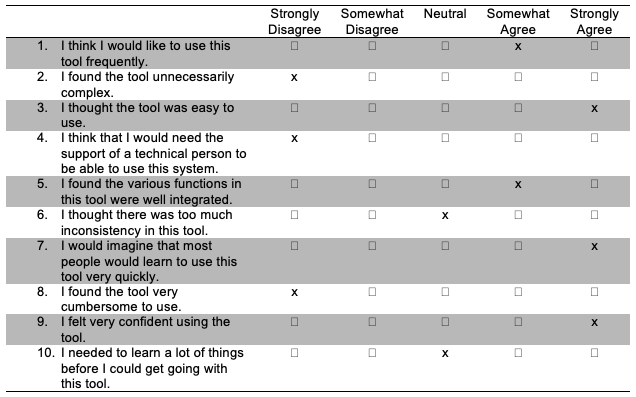
\includegraphics[width=0.95\textwidth]{graphics/sus_person6.png}
\end{center}

\textbf{Follow-up:}  
\begin{enumerate}
    \item \textbf{Was hat Ihnen am Tool am besten gefallen?}
    \begin{itemize}
        \item Möglichkeit kreativ zu sein.
    \end{itemize}

    \item \textbf{Gab es etwas, das verwirrend oder schwierig zu bedienen war?}
    \begin{itemize}
        \item Kurz verwirrt/irritiert, weil Wand „mitgegümmelt“ wurde.
    \end{itemize}

    \item \textbf{Fehlt etwas, das Sie erwartet oder gerne gehabt hätten? / Verbesserungsvorschläge}
    \begin{itemize}
        \item Bessere Stiftspitze (spitzer).  
        \item Anmerkung: Beamer-Qualität beachten.  
        \item Hintergrund nicht mit „gümmeln“, abhängig von Ausgangslage.  
        \item Feinerer Stiftkopf beim weissen Stift besser als beim schwarzen.  
        \item Sichtbarkeit der Taskleiste verwirrend (dachte, etwas aus Windows File Explorer holen zu müssen).  
        \item Gitternetz am Anfang unklar, ob man daran gebunden ist oder darüber hinaus malen kann.  
        \item Bei weiteren Tests am Anfang mehr Einweisung geben, damit Personen besseres Gefühl haben.
    \end{itemize}
\end{enumerate}

\clearpage
